\section{Introduction}
\label{openpsg:sec:introduction}

This chapter is the third step of the PSG line in the thesis.
Chapters~3 and~4 widened what a model can express within a fixed label space, first across the head and tail of the distribution and then through language priors. The remaining limit on control is the label space itself, since relations are still predicted from a predefined vocabulary.
The goal here is therefore to extend PSG to open-set relation prediction while retaining pixel-level grounding, so that the set of expressible relations is specified at inference time rather than fixed during training.


\begin{figure}[h]
    \centering
    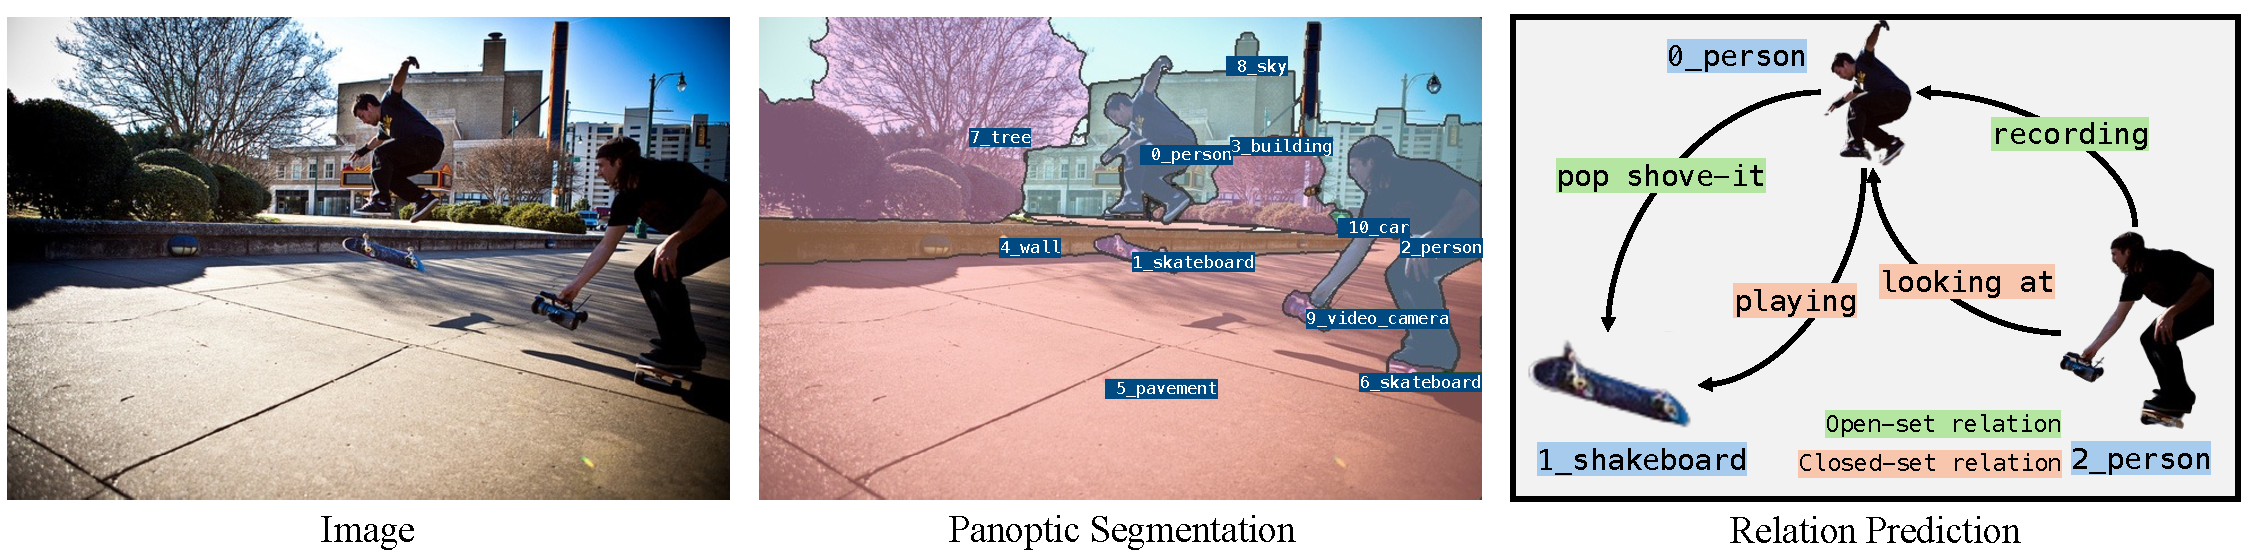
\includegraphics[width=1.0\linewidth]{Chapter5/Figures/vis.pdf}
    \caption{The left image is the input to our OpenPSG, the middle one displays the panoptic segmentation result, and the right one shows the predicted relations between objects.
    Our method can predict both known (close-set) relations, \eg, (0\_person, \textit{playing}, 1\_skateboard), (2\_person, \textit{looking at}, 0\_person), and unknown (open-set) relations, \eg, (0\_person, \textit{pop shove-it}, 1\_skateboard), (2\_person, \textit{recording}, 0\_person).}
    \label{openpsg:fig:open_figure}
\end{figure}


Panoptic scene graph generation (PSG)~\citep{yang2022panoptic} aims to segment objects within an image and recognize the relations among them, thereby constructing a panoptic scene graph for a structured understanding of the image.
Given its significant potential in applications such as visual question answering~\citep{hildebrandt2020scene}, image captioning~\citep{gao2018image, chen2020say}, and embodied navigation~\citep{singh2023scene}, PSG has attracted considerable attentions from researchers ever since its emerging~\citep{zhou2023hilo, wang2023pair, li2023panoptic, yang2023focusing, zhao2023textpsg, zhou2025vlprompt}.

Previous PSG methods, including those developed in Chapters~3 and~4, are only capable of predicting closed-set object and relation categories while failing to recognize objects/relations beyond predefined categories.
Recently, with the advent of large multimodal models (LMMs) such as CLIP~\citep{radford2021learning}, BLIP-2~\citep{li2023blip} \etc, a significant number of open-set prediction methods for object detection~\citep{du2022learning, zang2022open, lin2022learning, zhang2023simple, yao2023detclipv2} and segmentation~\citep{ghiasi2022scaling, liang2023open, zhang2023simple, yu2023towards} are introduced, attributing to LMMs' rich understanding of language and strong connections between vision and language.
Nevertheless, open-set prediction of relations has been largely unexplored so far.

Compared to open-set object detection and segmentation, open-set relation prediction is more complex: 
the model is required to both understand different objects and  recognize relations of object pairs based on their interactions; especially,  the computation of the latter can be exponentially increased.  
This chapter therefore focuses on open-set relation prediction as the missing component required for open-world PSG. 

LLMs~\citep{li2023blip, liu2024visual, zhu2023minigpt} have demonstrated exceptional semantic analysis and understanding abilities across various multimodal tasks.
In particular with the text processing, LMMs are not only good at interpreting on nouns (\ie  representing objects) but also pay considerable attention on predicates (\ie representing relations between objects), ensuring their generated contents to be sufficiently coherent~\citep{achiam2023gpt}.
Inspired by this, we propose the \textbf{Open}-set \textbf{P}anoptic \textbf{S}cene \textbf{G}raph Generation architecture, \textbf{OpenPSG}, leveraging the capabilities of LMMs for open-set relation prediction.

To this end, we utilize a large multimodal model (\eg, BLIP-2~\citep{li2023blip}) to achieve open-set relation prediction.
Specifically, our model comprises three parts.
First, the \textit{open-set panoptic segmenter}, we adapt an existing model (\eg, OpenSeeD~\citep{zhang2023simple}) which is capable of extracting open-set object categories, masks, and visual features from the whole image, forming object pairs and pair masks.
Second, the \textit{relation query transformer}, which has two functions: extracting visual features of object pairs based on pair masks and with a special focus on pair interactions; judging the potential relations between object pairs.
They are realized by two sets of queries, pair feature extraction query and relation existence estimation query.
Only those object pairs that are judged to likely have relations are fed into the third part, the \textit{multimodal relation decoder}.
This decoder directly inherits from the LMM to predict the open-set relations given an object pair in an auto-regressive manner, on condition of specifically-designed text instructions and pre-extracted pair visual features.

This chapter formulates open-set panoptic scene graph generation, enabling open-set prediction of both object masks and relations.
Extensive experiments demonstrate that our OpenPSG achieves state-of-the-art results in the closed-set setting and exhibits outstanding performance in the open-set setting.
Within the thesis, OpenPSG completes the structured-understanding progression from long-tail closed-set PSG (Chapter~3), to language-assisted closed-set PSG (Chapter~4), to open-world grounded relation prediction.
The next chapter starts Part~II and turns to control in visual generation.
